\documentclass[../../topologia_algebraica]{subfiles}
\begin{document}
\section{Producto ``smash''}\label{sec:producto_smash}

Las dos secciones anteriores me obligan a desarrollar una manera de calcular la suspensi\'on
reducida porque el lado izquierdo del ejercicio \ref{ej:11} se parece mucho a la definici\'on
\ref{def:grupo_fundamental_dimension_n}; quiero una manera de encontrar una relaci\'on
\[
  \begin{tikzcd}
    \Big[ (\Ss X,\star),(Y,y_0) \Big] \arrow[r,squiggly] & \Big[ (\Sn^n,1),(Y,y_0) \Big]=\pi_n(Y,y_0)
  \end{tikzcd}
\]

Resulta que la suspensi\'on se puede caracterizar mediante otra construcci\'on topol\'ogica:
el producto smash:

\begin{defin}
  Sean $(X,x_0)$ y $(Y,y_0)$ espacios basados, entonces su \emph{smash product} se define como
  el espacio cociente $X\times Y$ identificando $X\vee Y$ a un punto:
  \[
    X\wedge Y := (X\times Y)/_{X\vee Y}.
  \]
\end{defin}

\begin{nota}
  Recuerda que la discusi\'on que motiva el ejercicio \ref{ej:6} nos garantiza que $X\vee Y$ es
  homeomorfo al subespacio $(X\times\{y_0\})\cup (\{x_0\}\times Y)$ de $X\times Y$ y as\'i el
  smash product est\'a bien definido. Como consecuanecia de esto, puedo reescribir el smash
  product como:
  \[
    X\wedge Y := (X\times Y)/_{(X\times\{y_0\})\cup (\{x_0\}\times Y)}.
  \]
  La figura \ref{fig:smash_circulos} ilustra el proceso de identificaci\'on para obtener el
  smash product de dos c\'irculos.
\end{nota}

%%%%%%%%%%%%%%%%%%%%%%%%%%%%%%%%%%%%%%%%%%%%%%%%%%%%%%%%%%%%%%%%%%%%%%%%%%%%%%%%%%%%%%%%%%%%%%%%%%%
\begin{figure}
  \centering
  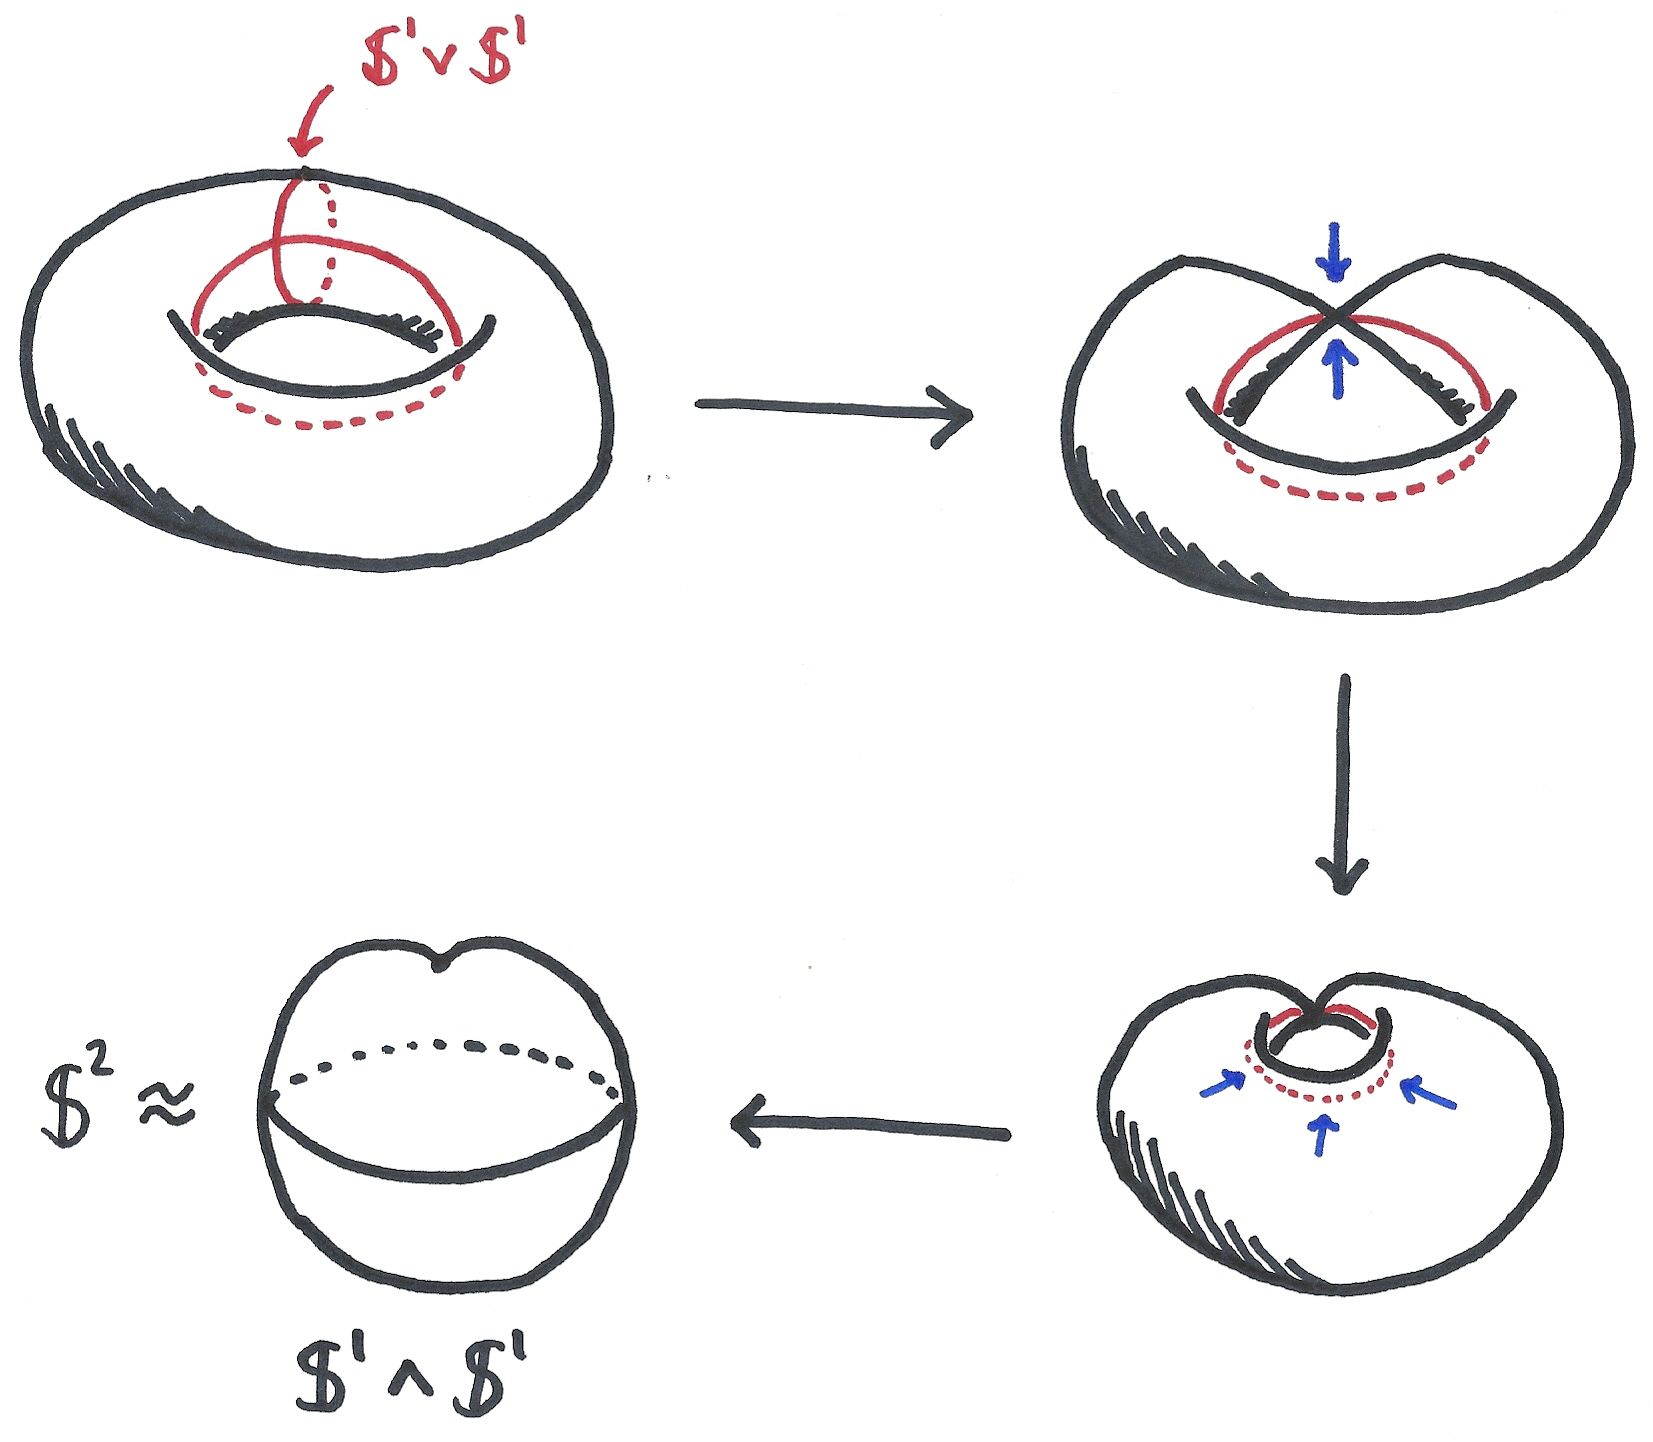
\includegraphics[scale=0.15]{smash_circulos}
  \caption{Construcci\'on de $\Sn^1\wedge\Sn^1$.}
  \label{fig:smash_circulos}
\end{figure}
%%%%%%%%%%%%%%%%%%%%%%%%%%%%%%%%%%%%%%%%%%%%%%%%%%%%%%%%%%%%%%%%%%%%%%%%%%%%%%%%%%%%%%%%%%%%%%%%%%%

La relaci\'on entre la suspensi\'on reducida y el smash product es evidente con el siguiente resultado:

\import{\directory}{ejercicios/9} %%%%%%%%%%%%%%%%%%%%%%%%%%%%%%%%%%%%%%%%%%%%%%%%%%%%%%% EJERICIO 9

La siguiente proposici\'on nos permite calcular la suspensi\'on reducida de cualquier esfera:

\begin{prop}\label{prop:smash_esferas}
  \[
    \Sn^1\wedge\Sn^n \approx \Sn^{n+1} \quad\forall n\geq 0
  \]
\end{prop}

\begin{proof}
  Encajo $\Sn^{n+1}\subset\RR^{n+2}$ como el conjunto de vectores unitarios y defino los hemisferios:
  \[
    \Sn^{n+1}_{\pm}:=\{(x_1,\ldots,x_{n+2})\in\Sn^{n+1}\mid \pm x_{n+2}>0\}.
  \]
  Tambi\'en encajo $\Sn^n\subset\Sn^{n+1}$ como
  \[
    \Sn^n:=\{(x_1,\ldots,x_{n+2})\in\Sn^{n+1}\mid x_{n+2}=0\},
  \]
  en particular $\Sn^{n+1}=\Sn^{n+1}_{+}\cup\Sn^{n+1}_-\cup\Sn^n$. Por \'ultimo encajo el disco
  unitario $\mathbb{D}^{n+1}\subset\RR^{n+2}$ como
  \[
    \mathbb{D}^{n+1}:=
    \{(x_1,\ldots,x_{n+2})\in\RR^{n+2}\mid \Sigma x_i^2\leq 1 \;\;\text{y}\;\; x_{n+2}=0\}.
  \]

  Ahora defino dos funciones $\rho_+$ y $\rho_-$ como $\rho_{\pm}:\mathbb{D}^{n+1}\ra\Sn^{n+1}_{\pm}$
  con regla de correspondencia:
  \[
    \rho_{\pm}(x_1,\ldots,x_{n+1},0)=\paren{x_1,\ldots,x_{n+1},\pm\sqrt{1-\sum_{i=1}^{n+1}x_i^2}}.
  \]
  Cada $\rho_{\pm}$ es continua porque $\sum x_i^2\leq 1$ y as\'i son composici\'on de funciones
  continuas. Adem\'as, son hoemoemorfismos porque ambas tienen el mismo inverso continuo: la
  proyecci\'on $\RR^{n+2}\ra\RR^{n+1}$ que iguala la \'ultima coordenada a 0 (estas $\rho's$ se parecen
  mucho a las cartas de la esfera $\Sn^{n+1}$ que la dotan de una estructura diferenciable, la
  \'unica diferencia es que las cartas tienen como dominio el disco abierto y como imagen al
  interior de los hemisferios, v\'ease el ejemplo \ref{ejemplo:cartas_hemisferios} de la secci\'on
  \ref{sec:variedades}).

  Sea $s_0=(1,0,\ldots,0)\in\Sn^n\subset\Sn^{n+1}$ el punto base de $\Sn^n$ y $\Sn^{n+1}$. Con esto
  defino la funci\'on $h:I\times\Sn^n\ra\Sn^{n+1}$ como:
  \[
    h(t,x):=
    \begin{cases}
      \rho_-(2tx+(1-2t)s_0) &\text{si}\;\; 0\leq t\leq\frac{1}{2}\\
      \rho_+(2(1-t)x+(2t-1)s_0) &\text{si}\;\; \frac{1}{2}\leq t\leq 1
    \end{cases}.
  \]
  Para probar que $h$ es continua basta ver que ambas partes coinciden en $t=\frac{1}{2}$. Como
  $x=(x_1,\ldots,x_{n+1},0)\in\Sn^n$ entonces $\Sigma x_i^2=1$ entonces:
  \[
    \rho_-(2\tfrac{1}{2}x+(1-2\tfrac{1}{2})s_0)=
    \rho_-(x)=
    (x_1,\ldots,x_{n+1},-\sqrt{1-\Sigma x_i^2})=
    (x_1,\ldots,x_{n+1},0)=x.
  \]
  Similarmente:
  \[
    \rho_+(2(1-\tfrac{1}{2})x+(2\tfrac{1}{2}-1)s_0)=
    \rho_+(x)=
    (x_1,\ldots,x_{n+1},\sqrt{1-\Sigma x_i^2})=
    (x_1,\ldots,x_{n+1},0)=x.
  \]
  Por lo tanto $h$ es continua.

  Adem\'as $h(0,x)=\rho_-(s_0)=s_0=\rho_+(s_0)=h(1,x)$, entonces $h$ se factoriza a trav\'es de:
  \[
    \begin{tikzcd}
      I\times\Sn^n \arrow[d,twoheadrightarrow,"\nu\times\Id_{\Sn^n}"'] \arrow[r,"h"] & \Sn^{n+1} \\
      \frac{I}{\partial I}\times\Sn^n \arrow[ur,dashed,"\bar{h}"'] &
    \end{tikzcd}
  \]
  Observa que, como $\Sn^n$ es compacto y Hausdorff y $\nu$ es una identificaci\'on, la funci\'on
  $\nu\times\Id_{\Sn^n}$ tambi\'en es una identificaci\'on.

  Lo \'unico que falta probar es que $\bar{h}$ se factoriza a trav\'es de
  \[
    \begin{tikzcd}
      \frac{I}{\partial I}\times\Sn^n \arrow[d,twoheadrightarrow,"\pi"'] \arrow[r,"\bar{h}"] & \Sn^{n+1}\\
      \frac{I/\partial I\times\Sn^n}{I/\partial I\vee\Sn^n} \arrow[ur,dashed,"\hat{h}"'] &
    \end{tikzcd}
  \]
  y que $\hat{h}$ es biyectiva. Estas dos cosas nos implican que $\hat{h}$ es un
  homeomorfismo ya que ser\'ia una funci\'on continua y biyectiva con dominio compacto y Hausdorff
  (ie. $ \frac{I/\partial I\times\Sn^n}{I/\partial I\vee\Sn^n}=\Sn^1\wedge\Sn^n$) y por lo tanto
  $\Sn^1\wedge\Sn^n\approx\Sn^{n+1}$. Lo que me falta lo pruebo en el siguiente ejercicio:

\import{\directory}{ejercicios/10} %%%%%%%%%%%%%%%%%%%%%%%%%%%%%%%%%%%%%%%%%%%%%%%%%%%%%% EJERICIO 10 
  
\end{proof}

Si junto el ejercicio \ref{ej:9} y la proposici\'on \ref{prop:smash_esferas}, obtengo una
f\'ormula para calcular la suspensi\'on reducida de cualquier esfera:

\begin{cor}\label{cor:suspension_esfera}
  \[
    \Ss\Sn^n\approx \Sn^{n+1}
  \] 
\end{cor}

Con este corolario puedo reescribir la definici\'on del grupo fundamental (como mencion\'e al
principio de esta secci\'on). Omito la notaci\'on de espacio basado: para toda $n\geq 1$ tengo
\[
  \pi_n(X,x_0)=\Big[ \Sn^n, X \Big]=
  \Big[ \Ss\Sn^{n-1},X \Big] \longleftrightarrow
  \Big[ \Sn^{n-1},\Omega X \Big]=
  \pi_{n-1}(\Omega X,e).
\]
En particular para $n=1$ concluyo que
\[
  \pi_1(X,x_0) \longleftrightarrow \pi_0(\Omega X, e).
\]
Esto quiere decir que el grupo fundamental de un espacio est\'a en biyecci\'on can\'onico
con las componentes conexas de su espacio de lazos (cf. proposici\'on \ref{pi_cero_componentes}).
Tiene sentido este hecho porque, de alguna manera, las homotop\'ias entre lazos funcionan como
trayectorias que las une.
\end{document}